% compile with XeLaTeX
\documentclass[dvipsnames,mathserif]{beamer}
\setbeamertemplate{footline}[frame number]
\usepackage[bigfiles]{pdfbase}
\usepackage{tikz}
\usepackage{animate}
\usepackage{listings}
\lstset{
  basicstyle=\ttfamily\scriptsize,  % Choose a basic font and size for the code
  breaklines=true,             % Enable line breaking
  keywordstyle=\color{blue},   % Color for keywords (like 'Function' in pseudocode)
  commentstyle=\color{green},  % Color for comments (if you include any)
  frame=single                 % Add a frame around the code
}
\usetheme{Darmstadt}
\definecolor{beamer@blendedblue}{rgb}{0.2,0.2,0.7}
% for RTL liste
\makeatletter
\newcommand{\RTListe}{\raggedleft\rightskip\leftm}
\newcommand{\leftm}{\@totalleftmargin}
\makeatother

% RTL frame title
\setbeamertemplate{frametitle}
{\vspace*{-1mm}
  \nointerlineskip
    \begin{beamercolorbox}[sep=0.3cm,ht=2.2em,wd=\paperwidth]{frametitle}
        \vbox{}\vskip-2ex%
        \strut\hskip1ex\insertframetitle\strut
        \vskip-0.8ex%
    \end{beamercolorbox}
}
% align subsection in toc
\makeatletter
\setbeamertemplate{subsection in toc}
{\leavevmode\rightskip=5ex%
  \llap{\raise0.1ex\beamer@usesphere{subsection number projected}{bigsphere}\kern1ex}%
  \inserttocsubsection\par%
}
\makeatother

% RTL triangle for itemize
\setbeamertemplate{itemize item}{\scriptsize\raise1.25pt\hbox{\donotcoloroutermaths$\blacktriangleleft$}} 

%\setbeamertemplate{itemize item}{\rule{4pt}{4pt}}

\defbeamertemplate{enumerate item}{square2}
{\LR{
    %
    \hbox{%
    \usebeamerfont*{item projected}%
    \usebeamercolor[bg]{item projected}%
    \vrule width2.25ex height1.85ex depth.4ex%
    \hskip-2.25ex%
    \hbox to2.25ex{%
      \hfil%
      {\color{fg}\insertenumlabel}%
      \hfil}%
  }%
}}

\setbeamertemplate{enumerate item}[square2]
\setbeamertemplate{navigation symbols}{}

\setbeamertemplate{caption}[numbered]
\begin{document}

\rightskip\rightmargin
\title{Autómata Off-Lattice: Bandadas de agentes autopropulsados}
\author[Di Toro, Catino, Chayer]{Camila Di Toro \and Kevin Catino \and Iván Chayer}
\institute{}
\date{}

\begin{frame}
\maketitle
\vfill
\centering{
    {Instituto Técnologico de Buenos Aires}
    \\
    $[72.27]$ Simulación de Sistemas
    \\
}
\end{frame}

\begin{frame}{Contenidos}
\footnotesize \tableofcontents
\end{frame}
\section{Introducción}

{
\setbeamercolor{background canvas}{bg=beamer@blendedblue!30}
\begin{frame}
  % frame contents here
    \centering
  \Huge
  Introducción
\end{frame}
}

% 
\begin{frame}

\frametitle{Sistema Real}
\begin{block}{Sistema Real}
Partículas auto-propulsadas
\end{block}

\begin{alertblock}{Objetivo}
Investigar su auto-organización a partir de su interacción.
\end{alertblock}

\end{frame}

%
\begin{frame}
\frametitle{Modelo de partículas auto-propulsadas}
\begin{columns}[T] % Align columns at the top
    \begin{column}{0.4\textwidth}
      \begin{center}
        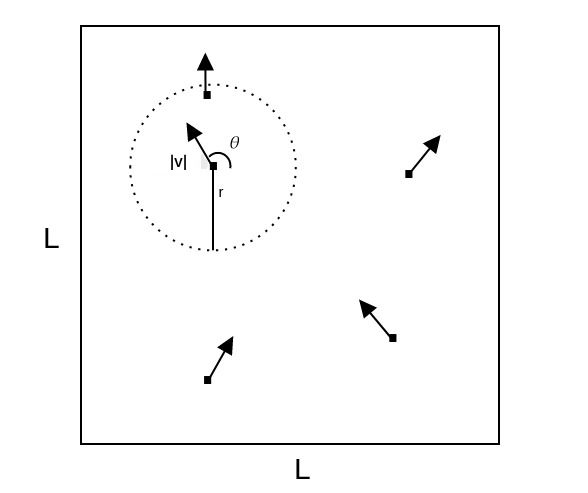
\includegraphics[width=\textwidth]{images/model.jpeg} % Replace with your image file 
      \end{center}
    \end{column}
    \begin{column}{0.6\textwidth}
        \footnotesize Reglas base del modelo:
        \begin{itemize}
            \item Cada partícula se desplaza en cada paso temporal
            \item Velocidad de módulo constante
            \item La dirección es un promedio de direcciones de velocidades vecinas en un radio de interacción "r" \footnote{El cálculo incluye el angulo de la propia partícula}
            \item Se adiciona ruido al cálculo de la dirección promedio    
        \end{itemize}
    \end{column}
\end{columns}
\end{frame}

% Opciones de items 
%
% La dirección se obtiene promediando dentro de un radio de interacción "r" las direcciones de las velocidades de las partículas vecinas.

%
\begin{frame}
\frametitle{Modelo de partículas auto-propulsadas}

Posición de la i-ésima partícula para cada tiempo $t$:
\begin{align}
     \boxed{x_i(t+1) = x_i(t) + v_i(t) \Delta t }
\end{align}

La dirección de la velocidad se obtiene a partir de la expresión:
\begin{align}
    \boxed{\theta (t+1) = \langle \theta (t) \rangle_r + \Delta \theta}
\end{align}

\begin{alertblock}{$\langle \theta (t) \rangle ~ y ~ \Delta \theta$}
Cálculo del promedio de los ángulos:

\begin{align}
 \langle \theta (t) \rangle_r  = atan2 \left[ \frac{\langle sin(\theta (t)) \rangle_r}{\langle cos(\theta (t)) \rangle_r} \right]
\end{align}

$\Delta \theta$ es el ruido y se obtiene de una distribución uniforme de intervalo $[-\frac{\eta}{2}, \frac{\eta}{2}]$

\end{alertblock}

\end{frame}


\section{Implementación}

{
\setbeamercolor{background canvas}{bg=beamer@blendedblue!30}
\begin{frame}
  % frame contents here
    \centering
  \Huge
  Implementación
\end{frame}
}

\begin{frame}
    \frametitle{Arquitectura}
    \begin{columns}[T] % Align columns at the top
        \begin{column}{0.6\textwidth}
          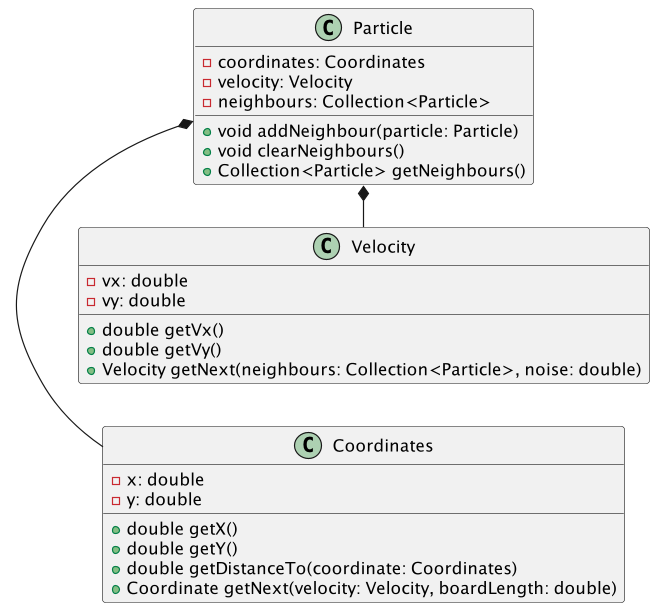
\includegraphics[width=\textwidth]{images/particle-diagram.png} 
        \end{column}
        \begin{column}{0.4\textwidth}
            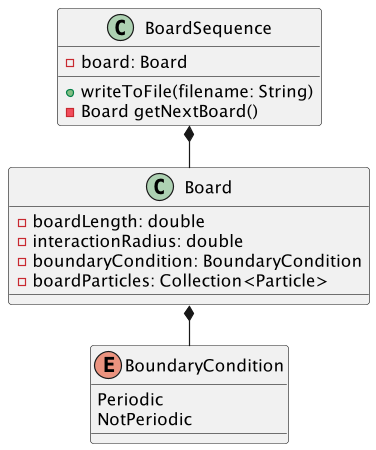
\includegraphics[width=\textwidth]{images/board-diagram.png} 
        \end{column}
    \end{columns}
\end{frame}

\begin{frame}
    \frametitle{Motor de simulación}
    \begin{block}{}
        Utiliza el método getNextBoard de la clase BoardSequence para avanzar en el tiempo y obtener el próximo Board.
    \end{block}

    \large Resumen de las operaciones realizadas:
    \begin{itemize}
            \item Cálculo de la nueva velocidad y posición 
            \item Se actualiza la velocidad y posición de la partícula
            \item Se recalcula las celdas en las que se encuentran las partículas
            \item Se obtienen los vecinos utilizando Cell Index Method
    \end{itemize}
    
\end{frame}

% \begin{frame}
%     \frametitle{Actualización de posición}
% \begin{lstlisting}[style=pseudocode, caption={Pseudocódigo para función getNext de clase Coordinates}]
% Function getNext(v: Velocity, boardLength: Real) -> Coordinates:

%     nextX = this.x + v.x
%     nextY = this.y + v.y
    
%     // wrapAxis es una funcion auxiliar que considera la condicion periodica de borde
%     nextX = wrapAxis(nextX, boardLength)
%     nextY = wrapAxis(nextY, boardLength)

%     return Coordinates(nextX, nextY)
% \end{lstlisting}

% \end{frame}

\begin{frame}[fragile]{Actualización de la posición}
  \begin{lstlisting}
Function getNext(v: Velocity, boardLength: Real) -> Coordinates:

    nextX = this.x + v.x
    nextY = this.y + v.y
    
    // se considera la condicion periodica de borde
    nextX = wrapAxis(nextX, boardLength)
    nextY = wrapAxis(nextY, boardLength)

    return Coordinates(nextX, nextY)
  \end{lstlisting}
\end{frame}

\begin{frame}[fragile]{Actualización de la velocidad}
  \begin{lstlisting}
getNext(neighbours: list<particle>, noise: double) -> Velocity:
    noiseValue = RandomBetween(-noise/2, noise/2)
    
    angles = new list
    for each particle IN neighbours:
        angle = arctan(particle.vy / particle.vx)
        angles.add(angle)

    selfAngle = arctan(this.velocity.y / this.velocity.x)
    angles.add(selfAngle)

    sinAvg = promedio de los senos en 'angles'
    cosAvg = promedio de los cosenos en 'angles'

    nextAngle = arctan(sinAvg / cosAvg) + noiseValue
    nextVx = cos(nextAngle) * modulo de v
    nextVy = sin(nextAngle) * modulo de v

    return Velocity(nextVx, nextVy)
  \end{lstlisting}
\end{frame}
\section{Simulaciones}

{
\setbeamercolor{background canvas}{bg=beamer@blendedblue!30}
\begin{frame}
  % frame contents here
    \centering
  \Huge
  Simulaciones
\end{frame}
}

\begin{frame}
\frametitle{Modelo Propuesto}
\begin{itemize}
    \item Partículas puntuales en una celda de lado \(L\) con condiciones periódicas.
    \item Velocidad constante \(v = 0.03\).
    \item Dirección \(\theta\).
    \item Radio de interacción \(r = 1\).
    \item \(N\) partículas en el sistema.
\end{itemize}
\end{frame}

\begin{frame}
\frametitle{Condiciones Iniciales}
\begin{itemize}
    \item Generación de \(N\) partículas aleatoriamente a \(t = 0\).
    \item Módulo de velocidad constante \(v = 0.03\).
    \item Direcciones \(\theta\) aleatorias, \(\theta \in [0, 2\pi]\).
\end{itemize}
\end{frame}

\begin{frame}
\frametitle{Comportamiento del Sistema}
\begin{itemize}
    \item Velocidad promedio normalizada \(v_a\) como observable.
    \[    v_a = \frac{1}{Nv} \left| \sum^{N}_{i=1} v_i \right|
\]
    \item Parámetros de interés: ruido \(\eta\) y densidad \(\rho = N / L^2\).
    \item \(v_a\) tiende a cero para desorden total y a 1 para partículas polarizadas.
\end{itemize}
\end{frame}

\begin{frame}
\frametitle{Simulaciones y Análisis}
\begin{itemize}
    \item Variación de \(v_a\) en función del ruido (\(\eta\)).
        \item Variación de \(v_a\) en función de la densidad (\(\rho\))
\end{itemize}
\end{frame}

\begin{frame}
\frametitle{Parámetros}
Comportamiento de \(v_a\) con ruido
    \begin{itemize}
    \item \(\eta \in [0, 5]\), \(N \in \{40, 100, 400\}\)
    \item Densidad constante \(\rho = 4\), ajuste \(L\) con \(N\).
    \end{itemize}
Comportamiento de \(v_a\) con densidad
    \begin{itemize}
    \item \(\rho \in [0, 10]\), \(L = 20\), \(\eta = 2.5\)
\end{itemize}

\end{frame}


\begin{frame}
\frametitle{Cálculo de \(v_a\) y Estado Estacionario}
\begin{itemize}
    \item Se calcula \(v_a\) cuando sistema esté estable.
    \item Se determina el tiempo estacionario con pruebas.
\end{itemize}
\end{frame}

\begin{frame}
\frametitle{Parámetros Constantes}
\begin{columns}
    \begin{column}{0.4\textwidth}
      \begin{center}
        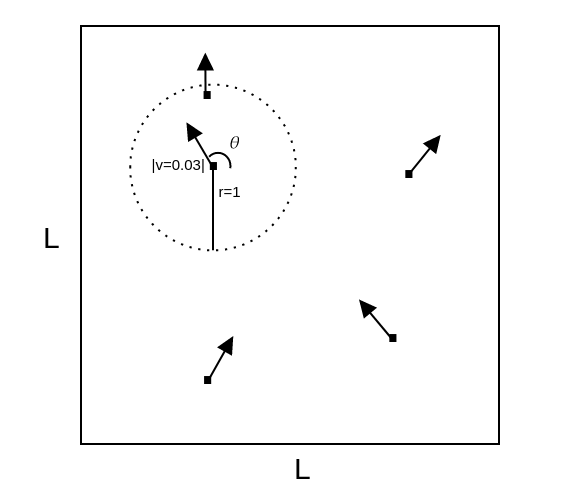
\includegraphics[width=\textwidth]{images/model-values.png} % Replace with your image file 
      \end{center}
    \end{column}
    \begin{column}{0.6\textwidth}
        \footnotesize
        \begin{itemize}
    \item Módulo velocidad: 0.03
    \item Radio interacción: 1
\end{itemize}
    \end{column}
\end{columns}

\end{frame}

\begin{frame}
\frametitle{Baja densidad}

\begin{columns}
    \begin{column}{0.7\textwidth}
      \begin{center}

\ifthenelse{\equal{\OUTPUT}{video}}
{\animategraphics[loop,controls,width=0.7\linewidth]{30}{animation/low_density/plot_}{0001}{1200}}
{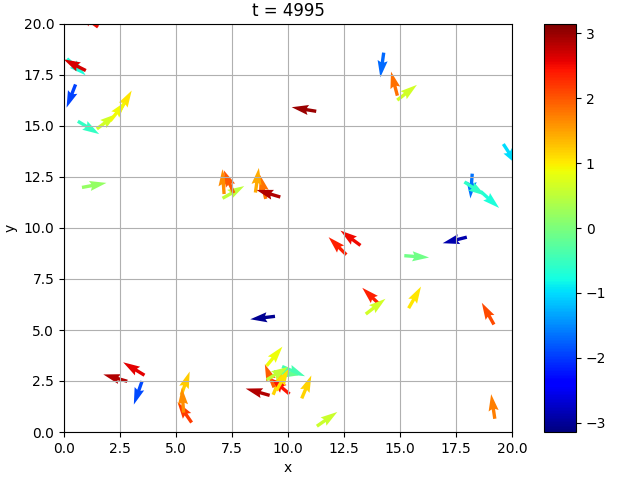
\includegraphics[width=0.7\linewidth]{animation/low_density/plot_1000.png}}

\end{center}
    \end{column}
    \begin{column}{0.3\textwidth}
\begin{center}
            \footnotesize
        \begin{itemize}
        \item \(L = 20\)
        \item \(\eta = 2.5\)
        \item \(N = 200\)
        \item \(\rho = 0.5\)
        \end{itemize}
\end{center}
    \end{column}
\end{columns}
\end{frame}

\begin{frame}
\frametitle{Alta densidad}

\begin{columns}
    \begin{column}{0.7\textwidth}
      \begin{center}
\ifthenelse{\equal{\OUTPUT}{video}}
{\animategraphics[loop,controls,width=0.7\linewidth]{30}{animation/high_density/plot_}{0001}{1200}}
{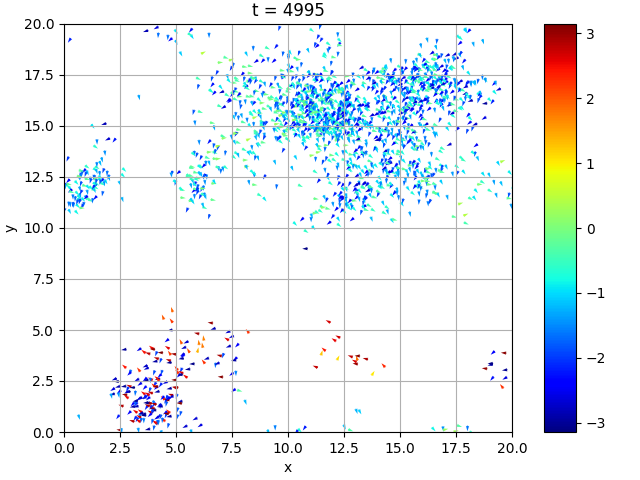
\includegraphics[width=0.7\linewidth]{animation/high_density/plot_1000.png}}
\end{center}
    \end{column}
    \begin{column}{0.3\textwidth}
\begin{center}
            \footnotesize
        \begin{itemize}
        \item \(L = 20\)
        \item \(\eta = 2.5\)
        \item \(N = 2000\)
        \item \(\rho = 5\)
        \end{itemize}
\end{center}
    \end{column}
\end{columns}
\end{frame}
\begin{frame}
\frametitle{Bajo ruido}

\begin{columns}
    \begin{column}{0.7\textwidth}
      \begin{center}
\ifthenelse{\equal{\OUTPUT}{video}}
{\animategraphics[loop,controls,width=0.7\linewidth]{30}{animation/low_noise/plot_}{0001}{1200}}
{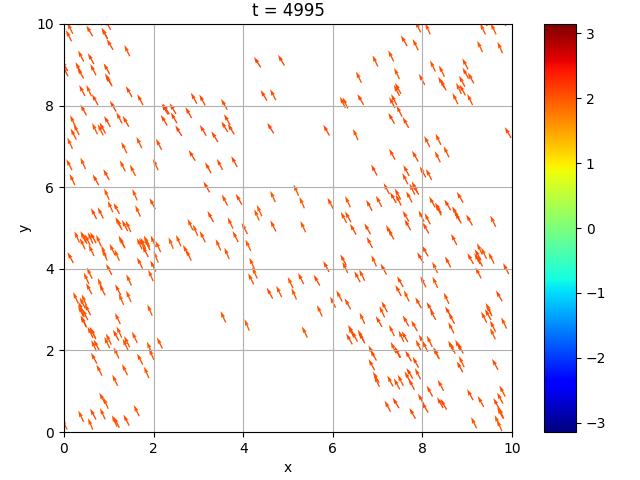
\includegraphics[width=0.7\linewidth]{animation/low_noise/plot_1000.png}}
\end{center}
    \end{column}
    \begin{column}{0.3\textwidth}
\begin{center}
            \footnotesize
        \begin{itemize}
        \item \(L = 10\)
        \item \(\eta = 0.1\)
        \item \(N = 400\)
        \item \(\rho = 4\)
        \end{itemize}
\end{center}
    \end{column}
\end{columns}
\end{frame}

\begin{frame}
\frametitle{Alto ruido}

\begin{columns}
    \begin{column}{0.7\textwidth}
      \begin{center}
\ifthenelse{\equal{\OUTPUT}{video}}
{\animategraphics[loop,controls,width=0.7\linewidth]{30}{animation/high_noise/plot_}{0001}{1200}}
{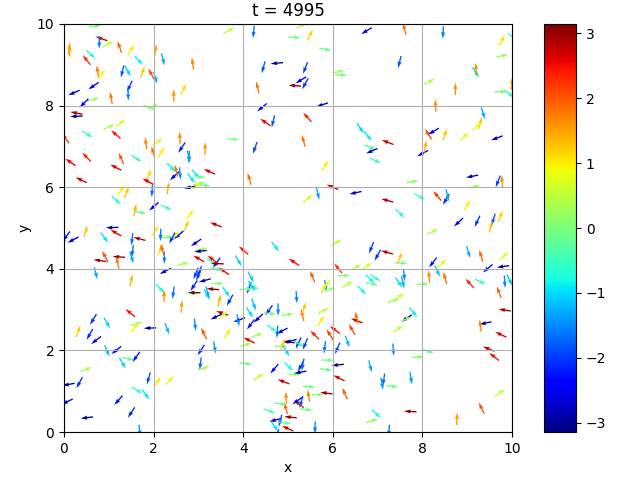
\includegraphics[width=0.7\linewidth]{animation/high_noise/plot_1000.png}}
\end{center}
    \end{column}
    \begin{column}{0.3\textwidth}
\begin{center}
            \footnotesize
        \begin{itemize}
        \item \(L = 10\)
        \item \(\eta = 5\)
        \item \(N = 400\)
        \item \(\rho = 4\)
        \end{itemize}
\end{center}
    \end{column}
\end{columns}
\end{frame}
















\section{Resultados}

{
\setbeamercolor{background canvas}{bg=beamer@blendedblue!30}
\begin{frame}
  % frame contents here
    \centering
  \Huge
  Resultados
\end{frame}
}

\begin{frame}
\frametitle{\(v_a\) en función del tiempo}
\begin{columns}
    \begin{column}{0.6\textwidth}
      \begin{center}
        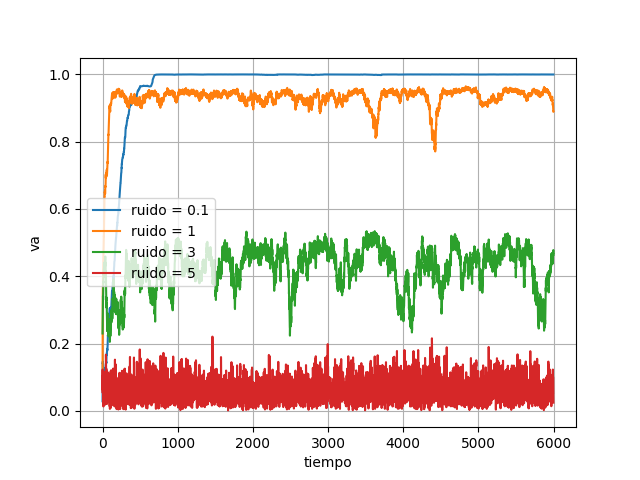
\includegraphics[width=\textwidth]{images/va-vs-tiempo-noise.png} % Replace with your image file 
      \end{center}
    \end{column}
    \begin{column}{0.4\textwidth}
                \footnotesize
       \begin{center}
                \begin{itemize}
        \item \(L = 10\)
        \item \(N = 400\)
        \end{itemize}
       \end{center}
    \end{column}
\end{columns}
        \begin{itemize}
        \item \(\eta \in \{3,5\}\): \(v_a\) no se estabiliza.
        \item \(\eta = 0.1\): \(v_a\) se estabiliza desde \(t \approx 700\).
                \item \(\eta = 1\): \(v_a\) se estabiliza desde \(t \approx 4500\).
        \end{itemize}
\end{frame}

\begin{frame}
\frametitle{\(v_a\) en función del tiempo}
\begin{columns}
    \begin{column}{0.6\textwidth}
      \begin{center}
        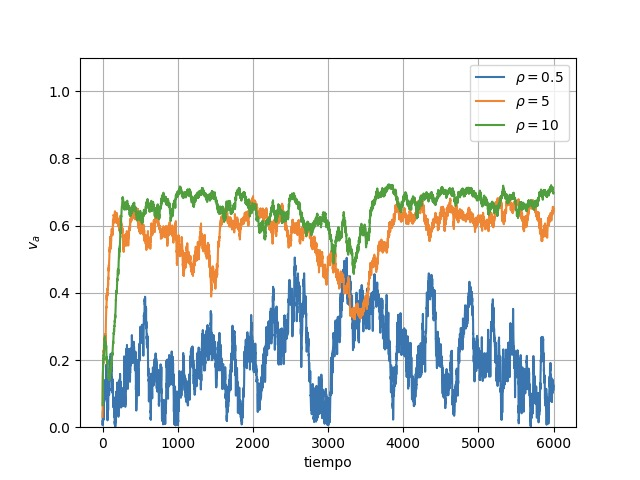
\includegraphics[width=\textwidth]{images/va-vs-tiempo-density.jpeg} % Replace with your image file 
      \end{center}
    \end{column}
    \begin{column}{0.4\textwidth}
\begin{center}
            \footnotesize
        \begin{itemize}
        \item \(L = 20\)
        \item \(\eta = 2.5\)
        \end{itemize}
\end{center}
    \end{column}
\end{columns}
        \begin{itemize}
        \item \(\rho \in \{5,10\}\): \(v_a\) se estabiliza desde \(t \approx 4000\)
        \item \(\rho = 0.5\): \(v_a\) no se estabiliza.
        \end{itemize}
\end{frame}

\begin{frame}
\frametitle{Cálculo de \(v_a\)}
Se decide utilizar el siguiente método:
 \begin{itemize}
        \item Si la variación de \(v_a\) en 50 iteraciones consecutivas es \(< 0.02\), se toma ese promedio.
        \item Si al llegar a la iteración 5000 no se cumplió la condición anterior, se calcula \(v_a\) como el promedio de las iteraciones 5001 a 6000.   
        \end{itemize}
\end{frame}
\begin{frame}
\frametitle{\(v_a\) en función del ruido}
\begin{columns}
    \begin{column}{0.6\textwidth}
      \begin{center}
        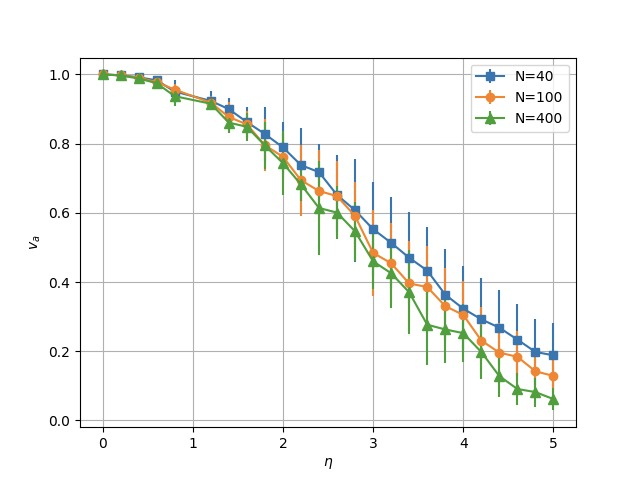
\includegraphics[width=\textwidth]{images/va-vs-ruido.jpeg} % Replace with your image file 
      \end{center}
    \end{column}
    \begin{column}{0.4\textwidth}
                \footnotesize
\begin{center}
            \begin{itemize}
        \item \(\rho = 4\)
        \end{itemize}
\end{center}
    \end{column}
\end{columns}
\end{frame}
\begin{frame}
\frametitle{\(v_a\) en función de la densidad}
\begin{columns}
    \begin{column}{0.6\textwidth}
      \begin{center}
        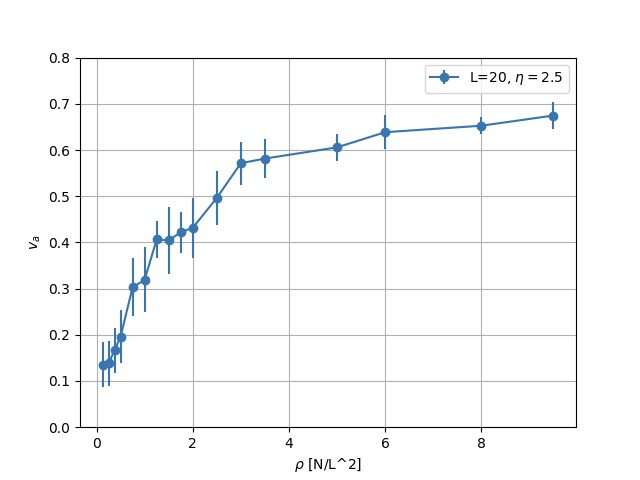
\includegraphics[width=\textwidth]{images/va-vs-density.jpeg} % Replace with your image file 
      \end{center}
    \end{column}
    \begin{column}{0.4\textwidth}
                \footnotesize
    \begin{center}
                \begin{itemize}
        \item \(\eta = 2.5\)
        \item \(  L = 20\)
        \end{itemize}
    \end{center}
    \end{column}
\end{columns}
\end{frame}
\section{Conclusiones}

{
\setbeamercolor{background canvas}{bg=beamer@blendedblue!30}
\begin{frame}
  % frame contents here
    \centering
  \Huge
  Conclusiones
\end{frame}
}

\begin{frame}

\frametitle{Conclusiones}
\begin{block}{}
    \begin{itemize}
        \item $v_a$ es un indicador de polarización de las partículas del sistema. 
    \end{itemize}
\end{block}

\begin{block}{Relación entre $\eta$ y $v_a$}
    \begin{align*}
        \uparrow \eta \implies \downarrow v_a
    \end{align*}
\end{block}

\begin{block}{Relación entre $\rho$ y $v_a$}
    \begin{align*}
        \uparrow \rho \implies \uparrow v_a
    \end{align*}
\end{block}

\end{frame}

\end{document}









